\documentclass[12pt, a4paper]{article}\usepackage[]{graphicx}\usepackage[]{color}
% maxwidth is the original width if it is less than linewidth
% otherwise use linewidth (to make sure the graphics do not exceed the margin)
\makeatletter
\def\maxwidth{ %
  \ifdim\Gin@nat@width>\linewidth
    \linewidth
  \else
    \Gin@nat@width
  \fi
}
\makeatother

\definecolor{fgcolor}{rgb}{0.345, 0.345, 0.345}
\newcommand{\hlnum}[1]{\textcolor[rgb]{0.686,0.059,0.569}{#1}}%
\newcommand{\hlstr}[1]{\textcolor[rgb]{0.192,0.494,0.8}{#1}}%
\newcommand{\hlcom}[1]{\textcolor[rgb]{0.678,0.584,0.686}{\textit{#1}}}%
\newcommand{\hlopt}[1]{\textcolor[rgb]{0,0,0}{#1}}%
\newcommand{\hlstd}[1]{\textcolor[rgb]{0.345,0.345,0.345}{#1}}%
\newcommand{\hlkwa}[1]{\textcolor[rgb]{0.161,0.373,0.58}{\textbf{#1}}}%
\newcommand{\hlkwb}[1]{\textcolor[rgb]{0.69,0.353,0.396}{#1}}%
\newcommand{\hlkwc}[1]{\textcolor[rgb]{0.333,0.667,0.333}{#1}}%
\newcommand{\hlkwd}[1]{\textcolor[rgb]{0.737,0.353,0.396}{\textbf{#1}}}%
\let\hlipl\hlkwb

\usepackage{framed}
\makeatletter
\newenvironment{kframe}{%
 \def\at@end@of@kframe{}%
 \ifinner\ifhmode%
  \def\at@end@of@kframe{\end{minipage}}%
  \begin{minipage}{\columnwidth}%
 \fi\fi%
 \def\FrameCommand##1{\hskip\@totalleftmargin \hskip-\fboxsep
 \colorbox{shadecolor}{##1}\hskip-\fboxsep
     % There is no \\@totalrightmargin, so:
     \hskip-\linewidth \hskip-\@totalleftmargin \hskip\columnwidth}%
 \MakeFramed {\advance\hsize-\width
   \@totalleftmargin\z@ \linewidth\hsize
   \@setminipage}}%
 {\par\unskip\endMakeFramed%
 \at@end@of@kframe}
\makeatother

\definecolor{shadecolor}{rgb}{.97, .97, .97}
\definecolor{messagecolor}{rgb}{0, 0, 0}
\definecolor{warningcolor}{rgb}{1, 0, 1}
\definecolor{errorcolor}{rgb}{1, 0, 0}
\newenvironment{knitrout}{}{} % an empty environment to be redefined in TeX

\usepackage{alltt}
\usepackage{geometry} % Page margins
\flushbottom
\geometry{
  a4paper,
  left=1cm,
  right=1.5cm,
  headsep = 1cm,            % controls distance to header from text
  headheight = 0.3cm,       % controls distance between header and page
  top=3cm,
  bottom=3cm,
  footskip=1.5cm            % controls distance to the footer from text
                            % increase this to "decrease" the footer
}
\parskip=8truept
\parindent=0mm

\usepackage{titlesec}
% \titlespacing{length1}{length2}{length3}
% length1 : how far left you'll make the heading go
% length2 : distance between previous section your section title. 
% length3 : distance between your section title and your body of text
\titlespacing*{\section}
{0pt}{0pt}{1.5mm} 
\titlespacing*{\subsection}
{0pt}{0cm}{1.5mm}
\titlespacing*{\subsubsection}
{0pt}{1.5mm}{1.5mm}

\newcommand{\horline}{\vspace{-6mm}\begin{flushleft}\mbox{}\hrulefill\mbox{}
\end{flushleft}\vspace{-6mm}} % make a horizontal line. 

% CLEARED
\usepackage{fancyhdr} % fancy header footer package

%\lfoot{\thepage}
%\rfoot{Mason Wong}

\usepackage{mathtools} %% helpful with equations and numbering. 
%\mathtoolsset{showonlyrefs}

%%%%%%%%%%%%%%%%% example of using fancy style for pages %%%%%%%%
%\fancypagestyle{vectors1.1}{
%\fancyhf{}
%\fancyhead[C]{top centre}
%\fancyhead[L]{top left}
%\fancyhead[R]{top right}
%\fancyfoot[C]{-\hspace{1.2mm}\thepage\hspace{1.5mm}-}
%\fancyfoot[L]{bottom left}
%\fancyfoot[R]{bottom right}
%\renewcommand{\headrulewidth}{0.4pt}
%\renewcommand{\footrulewidth}{0.1pt}
%}
% ex:
	% pagestyle{1-1} : all pages including this one
	% thispagestyle{1-1} : only this one
	% pagestyle{plain} : just a plain page number
	% pagestyle{empty} : produces empty head & feet & no pg num.

% get rid of header & footer
\fancypagestyle{myplain}{
\fancyhf{}
\renewcommand{\headrulewidth}{0pt}
\renewcommand{\footrulewidth}{0pt}
}
% get rid of header
\fancypagestyle{noheader}{
\fancyhf{}
\fancyfoot[C]{-\hspace{1.2mm}\thepage\hspace{1.5mm}-}
\renewcommand{\headrulewidth}{0pt}
\renewcommand{\footrulewidth}{0.4pt}
}
% 
\fancypagestyle{default}{
\fancyhf{}
\renewcommand{\headrulewidth}{0.4pt}
\renewcommand{\footrulewidth}{0.4pt}
\fancyhead[L]{STAT3022: Applied Linear Models}
\fancyhead[R]{Assignment 1}
\fancyfoot[C]{-\hspace{1.2mm}\thepage\hspace{1.5mm}-}
}

%%%%%%%%%%%%%%%%%%%%%%%%%%% Chapter layout %%%%%%%%%%%%%%
%\renewcommand{\thechapter}{\Roman{chapter}}
%\titleformat{\chapter}[display]
%{\bfseries\Large}
%{\filleft\MakeUppercase{\chaptertitlename} \Huge\thechapter}
%{4ex}
%{\titlerule
%\vspace{1ex}%
%\filright}
%[\vspace{1ex}%
%\titlerule]

%%%%%%%%%%%%%%%%%%%%%%%%% table of content layout %%%%%%%%%%%%%%%%%%%%%

%%%%%%%%%%%%%%% all of this is for the boxes %%%%%%%%%%%%%%%%%
\usepackage{tikz}
\usetikzlibrary{shadows} %defines shadows
\usepackage[framemethod=tikz]{mdframed}
%%%%%%%%%%%%%%%%%%%%%%%%%%%%%%%%%%%%%%%%%%%%%%%%%%%%%%%%%%%%%%
\global\mdfdefinestyle{myboxstyle}{%
shadow=true,
linecolor=black,
shadowcolor=black,
shadowsize=6pt,
nobreak=false,
innertopmargin=10pt,
innerbottommargin=10pt,
leftmargin=5pt,
rightmargin=5pt,
needspace=1cm,
skipabove=10pt,
skipbelow=15pt,
middlelinewidth=1pt,
afterlastframe={\vspace{5pt}},
aftersingleframe={\vspace{5pt}},
tikzsetting={%
draw=black,
very thick}
}
%%%%%%%%%%%%%%%%%%%%%%%%%%%%%%%%%%%%%%%%%%%%%%%%%%%%%%%%%%%%%
% framed box that allows page-breaks
\newmdenv[style=myboxstyle]{whitebox}
\newmdenv[style=myboxstyle,backgroundcolor=black!20]{graybox}
% framed box that CANNOT be broken at end of page
\newmdenv[style=myboxstyle,nobreak=true]{blockwhitebox}
\newmdenv[style=myboxstyle,backgroundcolor=black!20,nobreak=true]{blockgraybox}
% invisible box that CANNOT be broken at end of page
\newmdenv[nobreak=true,hidealllines=true]{blockbox}

%%%%%%%%%%%%%%%%%% tilde symbol for vectors %%%%%%%%%%%%%%%%%%
\DeclareMathAccent{\wtilde}{\mathord}{largesymbols}{"65}
% ex : \newcommand{\va}{\underaccent{\wtilde}{a}}

%%%%%%%%%%%%%%%%%%%% my new boxed thingies %%%%%%%%%%%%%%%%%%%%%%%%
\usetikzlibrary{shadows.blur} 
\newcommand{\mybox}[2]{
\begin{tikzpicture}
\node[draw=red, rectangle, line width=2pt, fill=yellow!30, rounded corners, inner sep=20pt, blur shadow={shadow xshift=1ex, shadow yshift=-1ex, shadow scale=1, shadow opacity=60, shadow blur radius=1.2ex}](temp){
\begin{minipage}{0.9\textwidth}
#2
\end{minipage}
};
\node[rectangle, rounded corners, fill=red, text=white, font={\bfseries}, right=5mm]  at (temp.north west) {#1};

\node[diamond, fill=red, text=white] at (temp.east) {$\spadesuit$};
\end{tikzpicture}
}

%%%%%%%%%%%%%%%%%% contradiction symbol %%%%%%%%%%%%%%%%%%%%%%%

\usepackage{tikz} %for the contradiction symbol
\usepackage{xifthen} %for the optional arument

\newcommand{\contradiction}{%

\begin{tikzpicture}[rotate=45,x=0.5ex,y=0.5ex]
\draw[line width=.2ex] (0,2) -- (3,2) (0,1) -- (3,1) (1,3) -- (1,0) (2,3) -- (2,0);
\end{tikzpicture}
}
%%%%%%%%%%%%%%%%%%%%%%%%% framing paragraphs %%%%%%%%%%%%%%%%%
\usepackage{mdframed} % allows for framing of words. 
%%%%%%%%%%%%%%%%%%%%%%%%%%%%%%%%%%%%%%%%%%%%%%%%%%%%%%%%%%%%%%%

%%%%%%%%%% squiggly arrow with some text over it %%%%%%%%%%%%%
% copied from internet. 
\usetikzlibrary{decorations.pathmorphing,shapes}

\newcounter{sarrow}
\newcommand\squigarrow[1]{%
\stepcounter{sarrow}%
\begin{tikzpicture}[decoration=snake]
\node (\thesarrow) {\strut#1};
\draw[->,decorate] (\thesarrow.south west) -- (\thesarrow.south east);
\end{tikzpicture}%
}

% ex : A \squigarrow{some text} B
% ex : C \squigarrow{\hbox to 0.9cm{}} D
% ex : E \squigarrow{\strut some text} F 

%%%%%%%%%%%%%%%%%%%%%%%% tabu package %%%%%%%%%%%%%%%%%%%%%%%%%
%\usepackage{tabu}

% example : changing column type and vertical spacing
% {\tabulinesep=1.2mm
% 	\begin{tabu}{CC}
%		1 & 2\\ \hline
% 		3 & 4\\ \hline
% 	\end{tabu}
% }

% example : look up latex colours for more colours. 
% \begin{tabu}{|CCCCCC|}
% \hline
% 	\rowcolor{LightCyan} 
% 	x & 0 & 1 & 2 & 3 & 4\\
% 	\rowcolor{babyblue}
% 	P(X = x) & 0.0625 & 0.25 & 0.375 & 0.25 & 0.0625\\
% 	\rowcolor{blizzardblue}
% 	\rowcolor{babyblue}
% 	P(X\le x) & 0.0625 & 0.3125 & 0.6875 & 0.9375 & 1\\ \hline
% \end{tabu}
%
%%%%%%%%%%%%%%%%%%% spacing (mu spacing)%%%%%%%%%%%%%%%%%%%%%%%%%
% \quad : 18mu 		% \, : 3/18 of quad 	% \: : 4/18 of quad
% \; : 5/18 of quad % \! : -3/18 of quad   % \ : normal space
% \qquad : two times \quad 

%%%%%%%%%%%%%%%%%%%% line over symbol %%%%%%%%%%%%%%%%%%%%%%%%%
%\mkern <num>mu : expands space where is it activated. 
%(i) when between words: eg "hello\mkern 18mu world" : will put
% 18 mu in between hello and world
% (ii) Since \overline is a box, when you do it inside overline
% \overline{\mkern 18mu \mathbb{R} \mkern 18mu} it will only
% move the R while making sure it's always in the box. 
% (iii) to test it out just have everything set to 0mu 

%\newcommand{\overbar}[1]{\mkern 0mu\overline{\mkern 0mu#1\mkern 0mu}\mkern 0mu}


% \overbar{size}{symbol} : size will dictate whether you want
% the overline to be shorter or longer. symbol is the symbol
% that you want with a line over it:
\newcommand{\overbar}[2]{\mkern -#1mu\overline{\mkern #1mu#2\mkern #1mu}\mkern -#1mu}
%%%%%%%%%%%%%%%%%%%%%%%%%%%%%%%%%%%%%%%%%%%%%%%%%%%%%%%%%%%%%%%

%%%%%%%%%%%%%%% code for expected value: %%%%%%%%%%%%%%%%%%%%%%
\DeclareRobustCommand{\bbone}{\text{\usefont{U}{bbold}{m}{n}1}}

\DeclareMathOperator{\EX}{\mathbb{E}}% expected value

\newcommand{\E}[1]{\EX[#1]}
%%%%%%%%%%%%%%%%%%%%%%%%%%%%%%%%%%%%%%%%%%%%%%%%%%%%%%%%%%%%%%%

%%%%%%%%%%%%%%%% Code for argument and cis %%%%%%%%%%%%%%%%%%%%%
\DeclareMathOperator{\Arg}{Arg}
\DeclareMathOperator{\cis}{cis}

%%%%%%%%%%%%%%%%%%%%%%% real and imaginary operators %%%%%%%%%%%
\DeclareMathOperator{\re}{Re}
\DeclareMathOperator{\im}{Im}

%%%%%%%%%%%%%%% code for variance %%%%%%%%%%%%%%%%%%%%%%%%%%%%
\newcommand{\Var}[1]{\mathrm{Var}[#1]}
\newcommand{\Cov}[1]{\mathrm{Cov}(#1)}
%%%%%%%%%%%%%%%%%%%%%%%%%%%%%%%%%%%%%%%%%%%%%%%%%%%%%%%%%%%%%%%

%%%%%%%%%%%%%%%% vareps %%%%%%%%%%%%%%%%%%%%%%%%%%%%%%%%%%%%
\newcommand{\vareps}{{\varepsilon}}

%%%%%%%%%%%%%%%%%%%%% integrals %%%%%%%%%%%%%%%%%%%%%%%%%%%%%%%
\usepackage{relsize}
% we can use
% \mathlarger{...}
% \int\limits_{a}^{b} something
\newcommand{\dx}{\, \text{d}x}
\newcommand{\dy}{\, \text{d}y}
\newcommand{\dz}{\, \text{d}z}
\newcommand{\dt}{\, \text{d}t}
\newcommand{\dm}{\, \text{d}m}
\newcommand{\dk}{\, \text{d}k}
\newcommand{\du}{\, \text{d}u}
\newcommand{\dv}{\, \text{d}v}

%%%%%%%%%%%%%%%%%%%%%% brackets %%%%%%%%%%%%%%%%%%%%%%%%%%%%%%
\newcommand{\rbrac}[1]{\left[#1\right]}
\newcommand{\brac}[1]{\left(#1\right)}
\newcommand{\cbrac}[1]{\left\{#1\right\}}

%%%%%%%%%%%%%%%%%%%%%%%%%%%%%%%%%%%%%%%%%%%%%%%%%%%%%%%%%%%%%
%%%%%%%%%%%%%%%%%%%%%%%%%%%%%%%%%%%%%%%%%%%%%%%%%%%%%%%%%%%%%
%%%%%%%%%%%%%%%%%%%%%%%%%%%%%%%%%%%%%%%%%%%%%%%%%%%%%%%%%%%%%

%%%%%%%%%%%%%% Commonly used commands and packages %%%%%%%%%%%%
\usepackage{amsmath} %math stuff
\usepackage{amssymb} % more math symbols
\usepackage{graphicx}
\usepackage{xcolor}
\usepackage{latexsym}
\usepackage{IEEEtrantools}
\usepackage{amsthm}
\usepackage{enumitem}
\definecolor{cadmiumgreen}{rgb}{0.0, 0.42, 0.24}
\newcommand{\tbf}[1]{{\bf #1}}
\newcommand{\bu}[1]{{\bf\underline{#1}}}
\newcommand{\red}[1]{{\color{red}#1}}
\newcommand{\vio}[1]{{\color{violet}#1}}
\newcommand{\teal}[1]{{\color{teal}#1}}
\newcommand{\blu}[1]{{\color{blue}#1}}
\newcommand{\bla}[1]{{\color{black}#1}}
\newcommand{\gre}[1]{{\color{cadmiumgreen}#1}}
\newcommand{\white}[1]{{\color{white}#1}}
\newcommand{\black}[1]{{\color{blacks}#1}}

\newcommand{\nn}{\mathbb{N}}
\newcommand{\zz}{\mathbb{Z}}
\newcommand{\qq}{\mathbb{Q}}
\newcommand{\rr}{\mathbb{R}}
\newcommand{\cc}{\mathbb{C}}
\newcommand{\abs}[1]{\left|#1\right|}
\newcommand{\inte}[1]{\noalign{\vspace{2\jot}\par{\noindent #1} \vspace{2\jot}}}
\newcommand{\interspace}[1]{
\inte{

\vspace{-2\baselineskip}

{

\setlength{\leftskip}{\textwidth - \linewidth}

#1

}

}
}
\newcommand{\st}{\,|\,}

%%%%%%%%%%%% Lebesgue outer measure and measure %%%%%%%%%%%%%%
\usepackage{suffix}
\newcommand{\lom}[1]{m_N{}^*\brac{#1}}
\WithSuffix\newcommand\lom*{m_N{}^*}
\newcommand{\lm}[1]{m_N\brac{#1}}
\WithSuffix\newcommand\lm*{m_N}

%%%%%%%%%%%%%%%%%%% new column types %%%%%%%%%%%%%%%%%%%%%%%%%%
\usepackage{array}  
% ex : math mode 
% \newcolumntype{C}{>{$}c<{$}} "prepend $ before every column and append $ before the end of every column"

%%%%%%%% tabular thick hline and column line %%%%%%%%%%%%%%%%%%
\makeatletter

% thick hline
\newcommand{\thickhline}{%
    \noalign {\ifnum 0=`}\fi \hrule height 1pt
    \futurelet \reserved@a \@xhline
}

% thick column. the @{.} is a separator between columns
\newcolumntype{"}{@{\hskip\tabcolsep\vrule width 1pt\hskip\tabcolsep}}

% thick left column (name not good : finger placement good)
\newcolumntype{a}{@{\vrule width 1.5pt\hskip\tabcolsep}}

% thick right column (name not good : finger placement good)
\newcolumntype{;}{@{\hskip\tabcolsep\vrule width 1.5pt}}

\makeatother

% ex: 
% \begin{tabular}{ac"c;} % the c's are the columns and the vertical stuff are a, " and ;

% 	\thickhline
% 	& 1 & 2 &\\
% 	& 3 & 4 &\\
% 	\thickhline
% \end{tabular}


%%%%%%%%%%%%%%%%%%%%%% tabular colouring columns %%%%%%%%%%%%%%
% include \usepackage{xcolor,colortbl} and \usepackage{array}

% ex: new column X and new column T. 
% \newcolumntype{X}[2]{>{\columncolor{#1}\centering}m{#2}}
% \newcolumntype{T}[2]{>{\columncolor{#1}\raggedright\arraybackslash}p{#2}}

% \begin{tabular}{|X{blue!20}{3cm}|T{green!20}{\textwidth -6cm}|}
% 	1 & 2\\
% \end{tabular}

%%%%%%%%%%%%%%%%%%%%%%% tabular colouring rows %%%%%%%%%%%%%%%%%
% ex:
% \definecolor{orange}{rgb}{0.93, 0.53, 0.18}
% \colorlet{darkorange}{orange!150}
%	\begin{tabular}{a p{3cm} " >{\raggedright\arraybackslash}				p{5cm} ; }
% 		\thickhline
% 		\rowcolor{darkorange!20}
% 		first word & second word \\ \thickhline
% 	\end{tabular}
%%%%%%%%%%%%%%%%%%%%%%%%% remark %%%%%%%%%%%%%%%%%%%%%%%%%%%%%

\newcommand{\rmk}[2][]{
	\ifthenelse{\equal{#1}{}}{

	\noindent \gre{\underline{Rmk}
	
	\vspace{-2ex}

	\begin{enumerate}[label=(\alph*)]
	#2
	\end{enumerate}
		}
	}{
	
	\noindent\gre{\underline{Rmk} (#1)
	
	\vspace{-2ex}

	\begin{enumerate}[label=(\alph*)]
	#2
	\end{enumerate}
		}
	}
}


%%%%%%%%%%%%%%%%%%%%%%%%%%%%%%%%%%%%%%%%%%%%%%%%%%%%%%%%%%%%%%%

%%%%%%%%%%%%%%%%%%%%%%%% listed examples %%%%%%%%%%%%%%%%%%%%%%
% variant 1 : named examples
% \eg[name for examples]{
%	\item eg 1
%	\item eg 2
%	\item eg 3
% }

% variant 2 : unnamed examples
% \eg{
%	\item eg 1
%	\item eg 2
%	\item eg 3
% }
\newcommand{\eg}[2][]{
	\ifthenelse{\equal{#1}{}}{
	\noindent \underline{\smash{Examples}}
	\begin{enumerate}[label=(\alph*)]
	#2
	\end{enumerate}
	}{
	\noindent \underline{\smash{Examples}} (#1)
	\begin{enumerate}[label=(\alph*)]
	#2
	\end{enumerate}
	}
}
%%%%%%%%%%%%%%%%%%%%%%%%%%%%%%%%%%%%%%%%%%%%%%%%%%%%%%%%%%%%%%%

%%%%%%%%%%%%%%%%%%%%%%%%%% ex %%%%%%%%%%%%%%%%%%%%%%%%%%%%%%%%%
% variant 1 : will produce ex1 underline
% \ex[1]
%	
% variant 2 : will produce ex (note the no number
% \ex
\newcommand{\ex}[1][]{%
	\ifthenelse{\equal{#1}{}}{
	\noindent{\underline{\raisebox{-0.35ex}{\text{\Large$\varepsilon$}}$\chi$}}
	}{
	\noindent{\underline{\raisebox{-0.35ex}{\text{\Large$\varepsilon$}}$\chi$\raisebox{-0.6ex}{$#1$}}}
	}
}

%%%%%%%%%%%%%%%%%%%%%%%%%%%%%%%%%%%%%%%%%%%%%%%%%%%%%%%%%%%%%%%

%%%%%%%%%%%%%%%%%%%%%%%%%% corollary %%%%%%%%%%%%%%%%%%%%%%%%%%
% variant 1 : name given
% \cor[name]{number}{what you wanna write}

% variant 2 : no name given
% \cor{number}{what you wanna write
\newcommand{\cor}[3][]{%
\ifthenelse{\equal{#1}{}}{
	\begin{graybox}
	\vspace{1ex}

	\blu{
		\noindent \underline{Cor #2}

		\noindent #3

	}
	
	\vspace{1ex}
	\end{graybox}
	}{
	\begin{graybox}
	\vspace{1ex}

	\blu{
		\noindent \underline{Cor #2} (#1)

		\noindent #3

	}
	
	\vspace{1ex}
	\end{graybox}
	}%
}
%%%%%%%%%%%%%%%%%%%%%%%%%%%%%%%%%%%%%%%%%%%%%%%%%%%%%%%%%%%%%%%

%%%%%%%%%%%%%%%%%%%%%%%%%%% theorem %%%%%%%%%%%%%%%%%%%%%%%%%%%
% variant 1 : name given
% \thm[name]{number}{what you wanna write}

% variant 2: no name given
% \thm{number}{what you wanna write}
\newcommand{\thm}[3][]{%
\ifthenelse{\equal{#1}{}}{
	\begin{graybox}
	\vspace{1ex}

	\blu{
		\noindent \underline{Thm #2}

		\noindent #3

	}
	
	\vspace{1ex}
	\end{graybox}
	}{
	\begin{graybox}
	\vspace{1ex}

	\blu{
		\noindent \underline{Thm #2} (#1)

		\noindent #3

	}
	
	\vspace{1ex}
	\end{graybox}
	}%
}
%%%%%%%%%%%%%%%%%%%%%%%%%%%%%%%%%%%%%%%%%%%%%%%%%%%%%%%%%%%%%%%

%%%%%%%%%%%%%%%%%%%%%%%%%%%% lemma %%%%%%%%%%%%%%%%%%%%%%%%%%%%% variant 1 : name given 
% \lem[name]{number}{stuff you wanna write}

% variant 2 : no name given
% \lem{number}{stuff you wanna write}
\newcommand{\lem}[3][]{%
\ifthenelse{\equal{#1}{}}{
	\begin{graybox}
	\vspace{1ex}

	\blu{
		\noindent \underline{Lemma #2}

		\noindent #3

	}
	
	\vspace{1ex}
	\end{graybox}
	}{
	\begin{graybox}
	\vspace{1ex}

	\blu{
		\noindent \underline{Lemma #2} (#1)

		\noindent #3

	}
	
	\vspace{1ex}
	\end{graybox}
	}%
}
%%%%%%%%%%%%%%%%%%%%%%%%%%%%%%%%%%%%%%%%%%%%%%%%%%%%%%%%%%%%%%%

%%%%%%%%%%%%%%%%%%%%%%%%%% proposition  %%%%%%%%%%%%%%%%%%%%%%%
% variant 1: name given 
% \prop[name]{number}{stuff you wanna write}

% variant 2 : no name given
% \prop{number}{stuff you wanna write}
\newcommand{\prop}[3][]{%
\ifthenelse{\equal{#1}{}}{
	\begin{graybox}
	\vspace{1ex}

	\blu{
		\noindent \underline{Prop #2}

		\noindent #3

	}
	
	\vspace{1ex}
	\end{graybox}
	}{
	\begin{graybox}
	\vspace{1ex}

	\blu{
		\noindent \underline{Prop #2} (#1)

		\noindent #3

	}
	
	\vspace{1ex}
	\end{graybox}
	}%
}
%%%%%%%%%%%%%%%%%%%%%%%%%%%%%%%%%%%%%%%%%%%%%%%%%%%%%%%%%%%%%%%

%%%%%%%%%%%%%%%%%%%%%%%%%% definition %%%%%%%%%%%%%%%%%%%%%%%%%
% variant 1 : name is given 
% \defn[name]{number}{stuff you wanna write}

% variant 2 : no name is given
% \defn{number}{stuff you wanna write}
\newcommand{\defn}[3][]{%
\ifthenelse{\equal{#1}{}}{
	\begin{graybox}
	\vspace{1ex}

	\blu{
		\noindent \underline{Def #2}

		\noindent #3

	}
	
	\vspace{1ex}
	\end{graybox}
	}{
	\begin{graybox}
	\vspace{1ex}

	\blu{
		\noindent \underline{Def #2} (#1)

		\noindent #3

	}
	
	\vspace{1ex}
	\end{graybox}
	}%
}
%%%%%%%%%%%%%%%%%%%%%%%%%%%%%%%%%%%%%%%%%%%%%%%%%%%%%%%%%%%%%%%

%%%%%%%%%%%%%%%%%%%%%%% normal working %%%%%%%%%%%%%%%%%%%%%%%%
% This is just for nomral working out. It's basically IEEE
% eqnarray*

\newcommand{\work}[1]{
\begin{IEEEeqnarray*}{rCl}
#1
\end{IEEEeqnarray*}
}

% priority is 
% 1. normalbaselineskip
% 2. inte
% 3. your equation

% \work{
% &&\\
% [-2\normalbaselineskip]
% 1 & = & 1\\
% 2 & = & 2\\
% 3 & = & 3\\
% [-3\normalbaselineskip]
% }

% \work{
% &&\\
% [-2\normalbaselineskip]
% 1 & = & 1\\
% 2 & = & 2\\
% \inte{note that these are words}
% 3 & = & 3\\
% 3 & = & 3\\
% [-3\normalbaselineskip]
% }

%%%%%%%%%%%%%%%%%%%%%%%%%%%%%%%%%%%%%%%%%%%%%%%%%%%%%%%%%%%%%%%

%%%%%%%%%% \align and starred variant \aligns %%%%%%%%%%%%%%%%%
\newcommand{\inter}[2]{
\setlength{\belowdisplayskip}{#1}%
\setlength{\abovedisplayskip}{#2}%
}

% \myalign{length of space above}{legnth of space below}{length of space horizontaly you wanna move}{align stuff}
\newcommand{\myalign}[4]{
	\gdef\nl{\hspace{#3} \\}
	{
	\inter{#1}{#2}
	\begin{align}
	#4
	\end{align}
	
	}
	
}
% \myaligns{length of space above}{legnth of space below}{length of space horizontaly you wanna move}{align stuff}
\newcommand{\myaligns}[4]{
	\gdef\nl{\hspace{#3} \\}
	{
	\inter{#1}{#2}
	\begin{align*}
	#4
	\end{align*}
	
	}
	
}

%%%%%%%%%%%%%%%%%%%%%%%%%%%% 	My QED symbols %%%%%%%%%%%%%%%%%%
\newcommand{\blackqed}{\rule{2mm}{2mm}}
\newcommand{\whiteqed}{
{\fboxsep=0pt\fcolorbox{black}{white}{\white{\blackqed}}
}}

\newcommand{\pf}[1]{
\emph{Proof:} #1 \hfill \blackqed
}

\newcommand{\sol}[1]{
\emph{Solution:} #1 \hfill \blackqed
}
%%%%%%%%%%%%%%%%%%%%%%%%%%%%%%%%%%%%%%%%%%%%%%%%%%%%%%%%%%%%%%%

%%%%%%%%%%%%%%% system of equations, centred at = %%%%%%%%%%%%%
% first argument = bracket size (a number)
% second argument = how much to push down (a number)
% third argument  = how much to push up (a number)
% fourth argument = your IEEEeqnarray stuff. 
\newcommand{\myeqn}[4]{
\begin{IEEEeqnarray*}{rrCl}
&&&\\
[#2\normalbaselineskip]
\smash{\left\{\IEEEstrut[#1\jot]\right.}\\
[#3\normalbaselineskip]
#4
\end{IEEEeqnarray*}
}

\newcommand{\myeqnarray}[4]{
\begin{IEEEeqnarraybox*}{rrCl}
&&&\\
[#2\normalbaselineskip]
\smash{\left\{\IEEEstrut[#1\jot]\right.}\\
[#3\normalbaselineskip]
#4
\end{IEEEeqnarraybox*}
}


%%%%%%%%%%%%%%%%%%%%%%%%%%%%%%%%%%%%%%%%%%%%%%%%%%%%%%%%%%%%%%%

%%%%%%%%%%%%%%%% system of equations, left aligned %%%%%%%%%%%%
\newcommand{\myeqnL}[4]{
\begin{IEEEeqnarray*}{rL}
&\\
[#2\normalbaselineskip]
\smash{\left\{\IEEEstrut[#1\jot]\right.}\\
[#3\normalbaselineskip]
#4
\end{IEEEeqnarray*}
}

\newcommand{\myeqnarrayL}[4]{
\begin{IEEEeqnarraybox*}{rL}
&\\
[#2\normalbaselineskip]
\smash{\left\{\IEEEstrut[#1\jot]\right.}\\
[#3\normalbaselineskip]
#4
\end{IEEEeqnarraybox*}
}
%%%%%%%%%%%%%%%%%%%%%%%%%%%%%%%%%%%%%%%%%%%%%%%%%%%%%%%%%%%%%%%

%%%%%%%%%%%%%%%% IEEEeqnarray and arraybox arguments %%%%%%%%%%
% IDENTIFIERS
% l : left math		c : centred math	r : right math
% L : left math with ords
% R : right math with ords
% C : centred math with ords
% s : left text		t : centred text	u : right text
% v : vertical rule		vv : two vertical rules
% V : double verticle rule		VV : two double vertical rules
% h : horizontal rule		HH : double horizontal rule
% x : empty					XX : empty math

% COLUMN SEPARATORS
% ! : -1/6em	% , : 1/6em		% : : 2/9em		% ; : 5/18em
% ' : 1em = \quad			% " : 2em = \qqad	
% . : 0.5\arraycolsep
% / : 1.0\arraycolsep		% ? : 2.0\arraycolsep	
% * : 0pt plus 1fil			% + : 1000pt minus 1000pt
% - : 0pt

%%%%%%%%%%%%%%%%%%% IEEEeqnarraybox examples %%%%%%%%%%%%%%%%%%
% example 1 : Making a tabular environment
% \begin{center}
% 	\begin{IEEEeqnarraybox}{t.t.t}
% 	\hline
%	\textbf{item} & \textbf{color} & \textbf{count} \\ \hline
%	cars & green & 17\\ \cline{1-3}
% 	trucks & red & 4\\ \cline{1-3}
%	bikes & blue & 25\\ \cline{1-3}
%	\end{IEEEeqnarraybox}
% \end{center}

% example 2 : Making piecewise functions. replacing with b or t aligns the bottome to the basleine and the top to the baseline respectively.  the \IEEEstrut[length] gives spacing
% \begin{equation}
% 	P_U(u) = \left\{
% 	\begin{IEEEeqnarraybox}[][c]{l's}
% 	\IEEEstrut[11pt]
% 	0.1 & if $u = 0$,\\
% 	0.3 & if $u = 1$,\\
% 	0.6 & if $u = 2$.
% 	\IEEEstrut
% \end{IEEEeqnarraybox}
% \right. \tag{vertically centred [c]}
% \end{equation}

% example 3 : makes a patchy table. We added the right appropriate spaces but it's patchy. This is the naive approach to doing things- see example 4 for a better example

% \begin{equation*}
% 	\begin{IEEEeqnarraybox}{c'c;v;c'c'c}
% 	D_1 & D_2 & & X_1 & X_2 & X_3 \\ \hline
% 	0 & 0 & & +1 & +1 & +1\\
% 	0 & 1 & & +1 & -1 & -1\\
% 	1 & 0 & & -1 & +1 & -1\\
% 	1 & 1 & & -1 & -1 & +1
% 	\end{IEEEeqnarraybox} \tag{naive: line breaks everywhere}
% \end{equation*}

% example 4 : the only difference frome example three is that this one has an extra optional argument. Remeber the second optional argument is for alignment (refer to example 2)

% \begin{equation*}
% 	\begin{IEEEeqnarraybox}[\IEEEeqnarraystrutmode][]{c'c;v;c'c'c}
% 	D_1 & D_2 && X_1 & X_2 & X_3 \\ \hline
% 	0 & 0 && +1 & +1 & +1\\
% 	0 & 1 && +1 & -1 & -1\\
% 	1 & 0 && -1 & +1 & -1\\
% 	1 & 1 && -1 & -1 & +1
% 	\end{IEEEeqnarraybox} \tag{using extra argument}
% \end{equation*}

% example 5 : added strutsizeadd next to strutmode. 10pt is adding 10 pt to the top of every row and 0pt means add 0pt to  the bottom of every row

% \begin{equation*}
% 	\begin{IEEEeqnarraybox}[ %
% 	\IEEEeqnarraystrutmode
% 	\IEEEeqnarraystrutsizeadd{10pt}{0pt}][]{c'c;v;c'c'c} 
% 	D_1 & D_2 && X_1 & X_2 & X_3\\ \hline
% 	0 & 0 && +1 & +1 & +1\\ 
% 	0 & 1 && +1 & -1 & -1\\ 
% 	1 & 0 && -1 & +1 & -1\\ 
% 	1 & 1 && -1 & -1 & +1\\ 
% 	\end{IEEEeqnarraybox} \tag{like ex4. included stutsizeadd}
% \end{equation*}

% example 6 : This example demonstrates you can't fully close that you'll have a little tail at the end of the box. Unsure how to fix this

% \begin{equation*}
% 	\begin{IEEEeqnarraybox}[
%\IEEEeqnarraystrutmode \IEEEeqnarraystrutsizeadd{1pt}{3pt}][]{v;c'c;v;c'c'c;v} \hline
% 	&D_1 & D_2 && X_1 & X_2 & X_3&\\ \hline
% 	&D_1 & D_2 && X_1 & X_2 & X_3& \\ \hline
% 	\end{IEEEeqnarraybox} \tag{another example}
%\end{equation*}
%%%%%%%%%%%%%%%%%%%%%%%%%%%%%%%%%%%%%%%%%%%%%%%%%%%%%%%%%%%%%%%

%%%%%%%%%%%%%%%%%%%%%%%%% IEEEeqnarray labelling %%%%%%%%%%%%%%
\makeatletter
\newcommand\ztag[1]{%
\def\@currentlabel{#1}%
\gdef\tmp{%
\addtocounter{equation}{-1}%
\def\theequation{#1}}%
\aftergroup\aftergroup\aftergroup\aftergroup\aftergroup\aftergroup
\aftergroup\aftergroup\aftergroup\aftergroup\aftergroup\aftergroup
\aftergroup\aftergroup\aftergroup\aftergroup\aftergroup\aftergroup
\aftergroup\aftergroup\aftergroup\aftergroup\aftergroup\aftergroup
\aftergroup\aftergroup\aftergroup\aftergroup\aftergroup\aftergroup
\aftergroup
\tmp}
\makeatother
% to use this \ztag{name} will give you the label "name" and \label{} will still work like normal. note, I put the \makeatother right after all the code, however, I think it should properly go at the start of the document. This might cause problems in the future. 

% ex : 
% \moveright 1in \vbox{
% 	\begin{work}{
% 		1 & = 1 \IEEEyesnumber \ztag{funny name} \label{1}
% 	}
% }

%%%%%%%%%%%%%%%%% to print commands %%%%%%%%%%%%%%%%%%%%%%%%%%%
% \verb+\mycommand+

% ex : \verb+\mylength+ is \the\mylength

%%%%%%%%%% save lengths after environment ends %%%%%%%%%%%%%%%%
% \global\mylength=\someLengthMacro

% ex : \global\mylength=\parindent

%%%%%%%%%%%%%%%%%%%%%%%%%% to show page layout %%%%%%%%%%%%%%%%%
% 1. use layout package in preamble
% 2. use the command \layout{} anywhere in the document
% 3. use the showframe package to see the dimensions visually

%%%%%%%%%%%%%%%%%%% captions without figures %%%%%%%%%%%%%%%%%
% use caption package 
% use the command \captionof{figure}{caption for image}

% ex:
% \begin{center}
% 	\includegraphics[scale=0.1]{p1}
% 	\captionof{figure}{this is the image p1}
% 	\label{p1}
% \end{center}
%%%%%%%%%%%%%%%%%%%%%%%%% cross references %%%%%%%%%%%%%%%%%%%%%
% 1. sections,  and figure can have a label. Something has to be before it: either a counter number or a caption
% 2. \ref{yourlabel} : references the counter
%	 \pageref{yourlabel} : references the page the label shows up on in the pdf. 	

%%%%%%%%%%%%%%%%%%%%%%%%% hyper links %%%%%%%%%%%%%%%%%%%%%%%%%%
% all you cross references will be linked. 
% use hyperref package (this should last package used)

% you can change things (though I think default is good):
% ex:
% \usepackage{hyperref}
% \hypersetup{
% 	colorlinks=true,
% 	linkcolor=blue,
% 	filecolor=magenta,
% 	urlcolor=cyan
% }

% To link addresses use : 
% 1. \href{<website>}{reference} : kinda discrete
% 2. \url{<website>} : straight up links you to the url 
% ex : for more info go to see \href{google.com}{this funny website}. alternatively just go straight to \url{google.com}

% To link local files:
% 1. \href{run:<some path>}{reference} : kinda discrete
% 2. \url{run:<some path>} : I'd much rather use href. also this has some problems. 
% ex : To remember how to solve quadratics, have a go at this \href{run:./file.txt}{worksheet}

% To link references manually:
% use the \hyperlink{label}{words} \hypertarget{label}{some other words}
% ex : click on the word \hyperlink{label1}{here} to jump tot he end of this \blindtext \hypertarget{label1}{paragraph}. 

% options to set in hypersetup:
% hyperindex (true): Makes the page numbers of index entries into hyperlinks.
% linktocpage (false): in TOC, makes the page numbers the link
% breaklinks (false): allows links to be broken into multiple lines
% colorlinks (false): links will be coloured instead
% linkcolor (red): color for links
% anchorcolor (black): color for target
% citecolor (green): color for bibliographies
% filecolor (cyan): color for files
% urlcolor (magenta): color for urls
% frenchlinks (false): uses small caps instead of colors for links. 
% citebordercolor (violet): color of box around bibliographies
% filebordercolor (cyan) : color of box around files
% linkbordercolor (red) : color of box around normal links. 
% urlbordercolor (violet) : color of box around urls. 
% menubordercolor (red) : color of box around menu links

%%%%%%%%%%%%% link between different documents %%%%%%%%%%%%%%
% in preamble:

% use hyperref package
% then AFTER hyperref, use the package: 
% \usepackage{nameref,zref-xr} 
% then the commands:
% \zxrsetup{toltxlabel}
% \zexternaldocument*{<path to document>} // no need for .tex

% in body:

% use : \ref{<label from previous document>} for the reference
% use : \namerf{<label from previous document>} for the name

% ex:

%%%%%% preamble %%%%%%
% \uespackage{hyperref}
% \usepackage{nameref, zref-xr}
% \zxrsetup{toltxlabel}
% \zexternaldocument*[boxes-]{../Latex-boxes-glue/practice-boxes}

%%%%%%% body %%%%%%%%%
% ...
% \ref{boxes-a} : number
% \nameref{boxes-a} : caption/ section name
% NOTE THAT IF WE DONT HAVE THE OPTIONAL ARGUMENT [boxes-] WE WOULDNT PUT IT IN FRONT OF OUR REFERENCE. IT'S JUST HELPFUL FOR ME. 

%%%%%%%%%%%% cont. arbitrary link between two documents %%%%%%
% include the hyperref package
% use the command pair in both documents:

% \hyperdef{label1}{label2}
% <some necessary text>
% \hyperref{<path to file>}{label1}{label2}{link that'll show up}

% though since label1 just has to match with label1, you can make label1 == label2 and define a new command

% ex : some shortcuts (put in both files)
% 1st arg : the label. needs to be the SAME in both docs
% 2nd arg : the path to the file. use a macro
% 3rd arg : the link that will be highlighted. can change color if you want to. 

% we need the kerns to ensure natural spacing. just try to think of it as a normal word (so you need spaces)

%\newcommand{\fileone}{<absolute path to file>}

%\newcommand{\twref}[3]{
%\newdimen\lengthofspace % length of space is 3.91663pt
%\lengthofspace=3.91663pt
%\hyperdef{#1}{#1}
%\kern -2\lengthofspace\hbox to 0pt{}
%\hyperref{#2}{#1}{#1}{#3\kern-\lengthofspace}
%}

% actual example: (needa do the same for the other file)
%\newcommand{\ephesiansOneFifteen}{../Ephesians1-15-23/Ephesians1-15-23}

% "refer back to \twref{lab1}{\ephesiansOneFifteen}{Ephesians 1:1--15} to recall how god loves us. 

%%%%%%%%%%%%%%%%%%%%%%%% rules and struts %%%%%%%%%%%%%%%%%%%%%%%
% \strut = \rule[-0.3\baselineskip]{0pt}{\baselineskip} where
% \rule[raise length]{width}{height}
% ex: 
%{
%\fboxsep=0pt

%\fbox{%
%\rule[0cm]{3pt}{\baselineskip} 
%\rule[0cm]{3pt}{\baselineskip}} : both stay at baseline

%\fbox{%
%\rule[1cm]{3pt}{\baselineskip} 
%\rule[0cm]{3pt}{\baselineskip}} : left one moves up by 1cm

%\fbox{%
%\rule[-\baselineskip]{3pt}{\baselineskip} 
%\rule[0cm]{3pt}{\baselineskip}} : left one moves down by a %baselineskip

%}

%%%%%%%%%%%%%%%%%%%%%%%% stack alignment %%%%%%%%%%%%%%%%%%%%%%%%
% use stackengine package
% 1. renew the stackalignment command to either l r or c
% ex : \renewcommand{\stackalignment}{c}

% 2. use \stackunder[length between first and second things]{first thing}{second thing}
% ex: \stackunder[0pt]{\rule{\texwidth}{0.5pt}}{hello}

% full ex:
% {
% 	\renewcommand{\stackalignment}{r}
% 	\stackunder[0pt]{\rule{\textwidth}{0.5pt}}{under word}
% }

%%%%%%%%%%%%%%%%%%%%%%%%%% making a nice title %%%%%%%%%%%%%%%%%%
% you needa put the strut there to make the box look nice and pretty. I instead use the definition of the strut and put it with the white so we can see it. 
% ex: 

% use stackengine package

% {
% \sffamily\Huge\noindent\fboxsep=0pt % the switches we use
% \renewcommand{\stackalignment}{r} % makes right aligned when we use \stackunder
% \stackunder[0pt]{\rule{\textwidth}{2pt}}{\colorbox{black}{{\color{white}\rule[-0.3\baselineskip]{2pt}{\baselineskip}T}}itle}
% }

%%%%%%%%%%%%%%%%%%%%%%%%%% Drawing right angles %%%%%%%%%
% use in tikz 
% ex : \dotMarkRightAngle[size=10pt](A, B, C);
% where A, B, C are given in clockwise order
\def\dotMarkRightAngle[size=#1](#2,#3,#4){%
 \draw ($(#3)!#1!(#2)$) -- 
       ($($(#3)!#1!(#2)$)!#1!90:(#2)$) --
       ($(#3)!#1!(#4)$);
% \path (#3) --node[circle,fill,inner sep=.5pt]{} ($($(#3)!#1!(#2)$)!#1!90:(#2)$);
}

\DeclareMathSymbol{*}{\mathbin}{symbols}{"03} % \ast
\DeclareMathSymbol{\ast}{\mathbin}{symbols}{"03}
% for the mathscr
\usepackage{mathrsfs}
% easier for bold symbols
\newcommand{\bs}[1]{\boldsymbol{#1}}
% partial derivatives
\newcommand{\partiald}[1]{\frac{\delta}{\delta#1}}
% second partial derivative
\newcommand{\partialdtwo}[1]{\frac{\delta^2}{\delta#1^2}}
% for estimators
\newcommand{\wh}[1]{\widehat{#1}}
% for examples
\newcommand{\gb}[1]{\greybox{#1}}
% text over arrow
\usepackage{mathtools}
% command for symbols under symbols
\newcommand{\under}[2]{\mathop{#1}\limits_{#2}}
% cancel to zero
\usepackage{cancel}
% Example: \cancelto{0}{x}

\titleformat{\section}{\normalfont\Large\bfseries}{}{0pt}{}
% for sets and curly letters
\newcommand{\cur}[1]{\mathcal{#1}}
\newcommand{\scr}[1]{\mathscr{#1}}

\usepackage{listings}
\definecolor{royalblue}{rgb}{0.25, 0.41, 0.88}
\definecolor{forestgreen}{rgb}{0.0, 0.27, 0.13}
\definecolor{rust}{rgb}{0.72, 0.25, 0.05}

\lstset{ 
  language=R,                     % the language of the code
  basicstyle=\footnotesize, % the size of the fonts that are used for the code
  numbers=left,                   % where to put the line-numbers
  numberstyle=\tiny\color{gray!150},  % the style that is used for the line-numbers
  stepnumber=1,                   % the step between two line-numbers. If it is 1, each line
                                  % will be numbered
  numbersep=5pt,                  % how far the line-numbers are from the code
  backgroundcolor=\color{gray!40},  % choose the background color. You must add \usepackage{color}
  showspaces=false,               % show spaces adding particular underscores
  showstringspaces=false,         % underline spaces within strings
  showtabs=false,                 % show tabs within strings adding particular underscores
  frame=single,                   % adds a frame around the code
  rulecolor=\color{black},        % if not set, the frame-color may be changed on line-breaks within not-black text (e.g. commens (green here))
  tabsize=2,                      % sets default tabsize to 2 spaces
  captionpos=b,                   % sets the caption-position to bottom
  breaklines=true,                % sets automatic line breaking
  breakatwhitespace=false,        % sets if automatic breaks should only happen at whitespace
  keywordstyle=\color{royalblue},      % keyword style
  commentstyle=\color{forestgreen},   % comment style
  stringstyle=\color{rust}      % string literal style
} 
\IfFileExists{upquote.sty}{\usepackage{upquote}}{}
\begin{document}
% refer to https://yihui.org/knitr/options/#code-decoration for more options


% (1) Remember that we want the default page style
% (2) but for this page we want an empty page style for the title 
% (3) we input our title 
% (4) we call a new page and reset the page counter to 1
\pagestyle{default}
\thispagestyle{empty}

\includegraphics[width=8cm]{./UsydLogo}

\vspace{1cm}


\horline
{\centering\bfseries \Large \textsc{STAT3023} Statiscal Inference

}
\horline

\vspace{3cm}

{\large \centering Lab Week 5

}

{\centering

\vspace{1cm}

Tutor: Wen Dai

SID: 470408326

\vspace{1cm}

School of Mathematics and Statistics

The University of Sydney

\vfill

Semester 2, 2021\newpage

}

\newpage
\setcounter{page}{1}

Consider the test of $H_0: \theta = \theta_0$ against $H_1 : \theta \neq \theta_0$ based on $X\thicksim f(. ; \gamma_0, \theta)$ where
\begin{align}
f\brac{x; \gamma, \theta} = 
\begin{cases}
\frac{1}{\Gamma\brac{\gamma}\theta^\gamma}x^{\gamma - 1}e^{-\frac{x}{\theta}} &\quad\text{for } x > 0 \\
0 &\quad\text{otherwise}
\end{cases}
\end{align}
that is $X$ has a gamma distribution with known shape parameter $\gamma_0$ but unknown scale parameter $\theta$.

\begin{enumerate}[label = {\bfseries \arabic*.}]
\item Consider first the exponential case where $\gamma_0 = 1$ and suppose the hypothesised value of the scale parameter (also the mean in this case) is $\theta_0 = 1$

  \begin{enumerate}[label = (\alph*)]
  \item The ``equal-tailed''test at level $\alpha$ rejects for $X \le a$ or $X \ge b$ where
    \begin{align}
    P_1\brac{X\le a} = P_1\brac{X\ge b} = \frac{\alpha}{2}
    \end{align}
    Taking $\alpha = 0.05$, determine the value sof \verb+a+ and \verb+b+ satisfying (2) above (\tbf{hint:} use \verb+qexp()+).
    
{\setlength{\leftskip}{3ex}
\tbf{Solution}

Since we take $\gamma_0 = 1$ and under the null $\theta_0 = 1$ we have that the the pdf is given by: 
$$ f(x) = e^{-x}\qquad\text{for } x > 0$$
\begin{knitrout}\footnotesize
\definecolor{shadecolor}{rgb}{0.969, 0.969, 0.969}\color{fgcolor}\begin{kframe}
\begin{alltt}
\hlstd{a} \hlkwb{=} \hlkwd{qexp}\hlstd{(}\hlnum{0.025}\hlstd{,} \hlkwc{rate} \hlstd{=} \hlnum{1}\hlstd{)}
\hlstd{b} \hlkwb{=} \hlkwd{qexp}\hlstd{(}\hlnum{0.975}\hlstd{,} \hlkwc{rate} \hlstd{=} \hlnum{1}\hlstd{)}
\hlkwd{c}\hlstd{(a, b)}
\end{alltt}
\begin{verbatim}
## [1] 0.02531781 3.68887945
\end{verbatim}
\end{kframe}
\end{knitrout}
}
    \item We shall plot the power function of the equal-tailed test. Define a vector of $\theta$-values: \verb+th=(250:1500)/1000+ and obtain a corresponding vector of values of the power (the proba- bility of rejecting) for each such $\theta$-value; that is:
    $$P_\theta \brac{X\le a} + P_\theta \brac{ X \ge b}$$
    Finally plot the power against \verb+th+ and add a horizontal dashed line at $\gamma = 0.05$. Add an informative heading, etc and remember to use \verb+type = 'l'+
    
    {\setlength{\leftskip}{3ex}
    
    \tbf{Solution}
    
    We plot the power function of the equal-tailed test. Note that for $P_\theta\brac{X \ge b}$ we note that $P_\theta\brac{X \ge b} = 1 - P_\theta\brac{X \le b}$. We alse use the \verb+abline(.)+ function to plot a horizontal line
    
\begin{knitrout}\footnotesize
\definecolor{shadecolor}{rgb}{0.969, 0.969, 0.969}\color{fgcolor}\begin{kframe}
\begin{alltt}
\hlstd{th} \hlkwb{=} \hlstd{(}\hlnum{250}\hlopt{:}\hlnum{1500}\hlstd{)}\hlopt{/}\hlnum{1000}
\hlstd{power} \hlkwb{=} \hlkwd{pexp}\hlstd{(a,} \hlkwc{rate} \hlstd{=} \hlnum{1}\hlopt{/}\hlstd{th,} \hlkwc{lower.tail} \hlstd{=} \hlnum{TRUE}\hlstd{)} \hlopt{+} \hlkwd{pexp}\hlstd{(b,} \hlkwc{rate} \hlstd{=} \hlnum{1}\hlopt{/}\hlstd{th,} \hlkwc{lower.tail} \hlstd{=} \hlnum{FALSE}\hlstd{)}
\hlcom{# Plot theta against the power:}
\hlkwd{plot}\hlstd{(th, power,} \hlkwc{type} \hlstd{=} \hlstr{"l"}\hlstd{,} \hlkwc{main} \hlstd{=} \hlstr{"Power of two tail test"}\hlstd{)}
\hlcom{# add a horizontal dashed line at gamma = 0.05}
\hlkwd{abline}\hlstd{(}\hlkwc{h} \hlstd{=} \hlnum{0.05}\hlstd{,} \hlkwc{lty} \hlstd{=} \hlnum{2}\hlstd{)}
\end{alltt}
\end{kframe}

{\centering 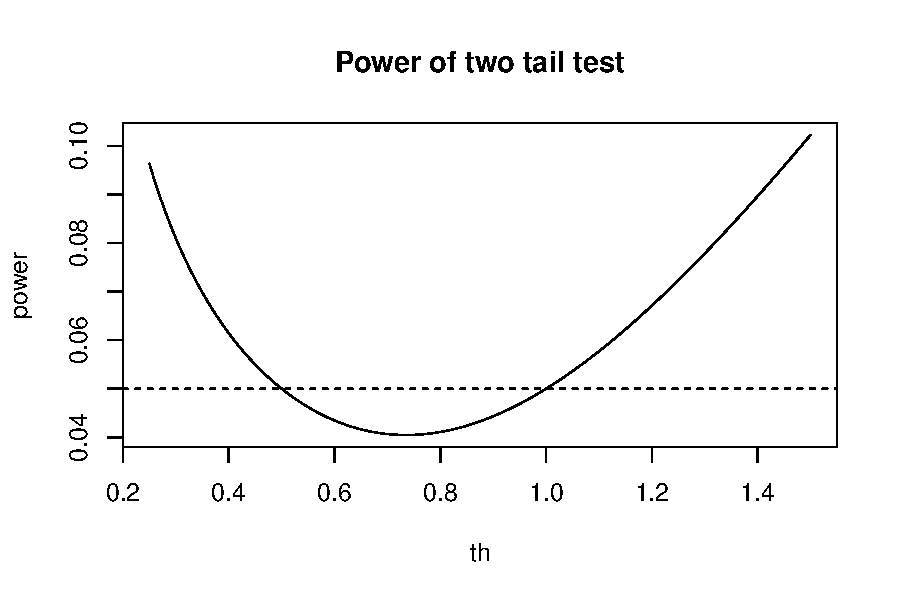
\includegraphics[width=\maxwidth]{figure/unnamed-chunk-3-1} 

}


\end{knitrout}
    
    }
    \item This is a 1-parameter exponential family with sufficient statistic $X$ and so (since it is continuous) the \textit{uniformly most powerful unbiased} (UMPU) test is of the form
    \begin{align}
    \delta\brac{X} = 
      \begin{cases}
      1 &\qquad\text{for } X \ge d \\
      0 &\qquad\text{for } c < X < d\\
      1 &\qquad \text{for } X \le c
      \end{cases}
    \end{align}
Where $c$ and $d$ are chosen so that:
  \begin{align}
    \E_{\theta_0}\rbrac{\delta\brac{X}} = \alpha
  \end{align}
  \begin{align}
  \E_{\theta_0}\rbrac{X\delta\brac{X}} = \alpha\E_{\theta_0}\brac{X} = \alpha
  \end{align}
  Since $\E_{\theta_0}\brac{X} = 1$. We show in a tutorial exercise these are equivalent to
  \begin{align*}
  1 - e^{-c} + e^{-d} & = \alpha \\
  ce^{-c} & = de^{-d}
  \end{align*}
  From the first equation we get:
  \begin{align*}
  e^{-d} & = \alpha - 1 + e^{-c} \\
  \implies d & = -\log \rbrac{\alpha -1 + e^{-c}}
  \end{align*}
  Hence, once $c$ is determined we can compute $d$. To determine $c$ we need to solve the equation:
  \begin{align*}
  ce^{-c} - de^{-d} = ce^{-c} + \cbrac{\log \rbrac{\alpha - 1 + e^{-c}}}\rbrac{\alpha - 1 + e^{-c}} = 0
  \end{align*}
  We can use the R function \verb+uniroot()+ to determine c \textit{numerically}.
    \begin{enumerate}[label=(\roman*)]
      \item Write an R function which computes the middle member of the equation above (i.e. the function whose root we wish to find).
      
      {\setlength{\leftskip}{3ex}
      \tbf{Solution}
      
      We write a function which computes the root $c$ to the equation 
      $$ce^{-c} + \cbrac{\log \rbrac{\alpha - 1 + e^{-c}}}\rbrac{\alpha - 1 + e^{-c}} = 0$$
\begin{knitrout}\footnotesize
\definecolor{shadecolor}{rgb}{0.969, 0.969, 0.969}\color{fgcolor}\begin{kframe}
\begin{alltt}
\hlstd{fn} \hlkwb{=} \hlkwa{function}\hlstd{(}\hlkwc{c}\hlstd{,} \hlkwc{alpha}\hlstd{) \{}
    \hlstd{term} \hlkwb{=} \hlstd{alpha} \hlopt{-} \hlnum{1} \hlopt{+} \hlkwd{exp}\hlstd{(}\hlopt{-}\hlnum{1} \hlopt{*} \hlstd{c)}
    \hlkwd{return}\hlstd{(c} \hlopt{*} \hlkwd{exp}\hlstd{(}\hlopt{-}\hlstd{c)} \hlopt{+} \hlstd{(}\hlkwd{log}\hlstd{(term)} \hlopt{*} \hlstd{term))}
\hlstd{\}}
\end{alltt}
\end{kframe}
\end{knitrout}
      
      }
      \item Noting that $c$ can be no bigger than the lower 0.05-quantile of the exponential(1) distribution, execute a certain command involving \verb+eps = 1e-5+. Note: the use of \verb+eps+ here is to stay away from the upper bound, since there the function is trying to evaluate \verb+log(0)+
\begin{knitrout}\footnotesize
\definecolor{shadecolor}{rgb}{0.969, 0.969, 0.969}\color{fgcolor}\begin{kframe}
\begin{alltt}
\hlstd{eps} \hlkwb{=} \hlnum{1e-05}
\hlkwd{uniroot}\hlstd{(}\hlkwc{f} \hlstd{= fn,} \hlkwc{lower} \hlstd{=} \hlnum{0}\hlstd{,} \hlkwc{upper} \hlstd{=} \hlkwd{qexp}\hlstd{(}\hlnum{0.05}\hlstd{)} \hlopt{-} \hlstd{eps,} \hlkwc{alpha} \hlstd{=} \hlnum{0.05}\hlstd{)}
\end{alltt}
\begin{verbatim}
## $root
## [1] 0.04235629
## 
## $f.root
## [1] -3.187136e-05
## 
## $iter
## [1] 4
## 
## $init.it
## [1] NA
## 
## $estim.prec
## [1] 6.103516e-05
\end{verbatim}
\end{kframe}
\end{knitrout}
      \item Write an R function which takes as an argument the level \verb+alpha+ and returns a list with elements \verb+c+ and \verb+d+, corresponding to the desired values $c$ and $d$ defining the UMPU test (3) above for $\theta_0 = 1$ and $\alpha = 0.05$
      
      {\setlength{\leftskip}{3ex}
      
      \tbf{Solution}
      
      We write a function \verb+expon.umpu+ (exponential uniformly most powerful unbiased test) which takes in $\alpha$ and returns the optimal $c$ and $d$ which solve the above equations. 
      
\begin{knitrout}\footnotesize
\definecolor{shadecolor}{rgb}{0.969, 0.969, 0.969}\color{fgcolor}\begin{kframe}
\begin{alltt}
\hlstd{expon.umpu} \hlkwb{=} \hlkwa{function}\hlstd{(}\hlkwc{alpha}\hlstd{) \{}
    \hlstd{eps} \hlkwb{=} \hlnum{1e-08}
    \hlstd{c} \hlkwb{=} \hlkwd{uniroot}\hlstd{(}\hlkwc{f} \hlstd{= fn,} \hlkwc{lower} \hlstd{=} \hlnum{0}\hlstd{,} \hlkwc{upper} \hlstd{=} \hlkwd{qexp}\hlstd{(alpha)} \hlopt{-} \hlstd{eps,} \hlkwc{alpha} \hlstd{= alpha)}\hlopt{$}\hlstd{root}
    \hlstd{term} \hlkwb{=} \hlstd{alpha} \hlopt{-} \hlnum{1} \hlopt{+} \hlkwd{exp}\hlstd{(}\hlopt{-}\hlstd{c)}
    \hlstd{d} \hlkwb{=} \hlopt{-}\hlkwd{log}\hlstd{(term)}
    \hlkwd{list}\hlstd{(}\hlkwc{c_val} \hlstd{= c,} \hlkwc{d_val} \hlstd{= d)}
\hlstd{\}}
\hlkwd{expon.umpu}\hlstd{(}\hlnum{0.05}\hlstd{)}
\end{alltt}
\begin{verbatim}
## $c_val
## [1] 0.04235611
## 
## $d_val
## [1] 4.764356
\end{verbatim}
\end{kframe}
\end{knitrout}
      
      }
    \end{enumerate}
  \item Recreate your plot from part (b) above and add to it a red curve of the power of the UMPU test. Add an informative heading and legend. \tbf{Comment} on what feature of the plot indicates that the UMPU test is unbiased. The power function of the UMPU test never goes below the 0.05 level, thus it is unbiased.
  
  {\setlength{\leftskip}{3ex}
  \tbf{Solution}
  
  We now plot the power of the UMPU test in red:
  
\begin{knitrout}\footnotesize
\definecolor{shadecolor}{rgb}{0.969, 0.969, 0.969}\color{fgcolor}\begin{kframe}
\begin{alltt}
\hlstd{th} \hlkwb{=} \hlstd{(}\hlnum{250}\hlopt{:}\hlnum{1500}\hlstd{)}\hlopt{/}\hlnum{1000}
\hlcom{# for the two tailed test}
\hlstd{power} \hlkwb{=} \hlkwd{pexp}\hlstd{(a,} \hlnum{1}\hlopt{/}\hlstd{th)} \hlopt{+} \hlkwd{pexp}\hlstd{(b,} \hlnum{1}\hlopt{/}\hlstd{th,} \hlkwc{lower.tail} \hlstd{=} \hlnum{FALSE}\hlstd{)}
\hlkwd{plot}\hlstd{(th, power,} \hlkwc{type} \hlstd{=} \hlstr{"l"}\hlstd{,} \hlkwc{main} \hlstd{=} \hlstr{"testing for an exponential mean"}\hlstd{)}
\hlkwd{abline}\hlstd{(}\hlkwc{h} \hlstd{=} \hlnum{0.05}\hlstd{,} \hlkwc{lty} \hlstd{=} \hlnum{2}\hlstd{)}
\hlcom{# for the uniformly most powerful test:}
\hlstd{umpu} \hlkwb{=} \hlkwd{expon.umpu}\hlstd{(}\hlnum{0.05}\hlstd{)}
\hlstd{umpu.power} \hlkwb{=} \hlkwd{pexp}\hlstd{(umpu}\hlopt{$}\hlstd{c,} \hlnum{1}\hlopt{/}\hlstd{th)} \hlopt{+} \hlkwd{pexp}\hlstd{(umpu}\hlopt{$}\hlstd{d,} \hlnum{1}\hlopt{/}\hlstd{th,} \hlkwc{lower.tail} \hlstd{=} \hlnum{FALSE}\hlstd{)}
\hlkwd{lines}\hlstd{(th, umpu.power,} \hlkwc{col} \hlstd{=} \hlstr{"red"}\hlstd{)}
\hlkwd{legend}\hlstd{(}\hlstr{"top"}\hlstd{,} \hlkwc{legend} \hlstd{=} \hlkwd{c}\hlstd{(}\hlstr{"Power of equal-tailed test"}\hlstd{,} \hlstr{"power of UMPU test"}\hlstd{),} \hlkwc{col} \hlstd{=} \hlkwd{c}\hlstd{(}\hlstr{"black"}\hlstd{,} \hlstr{"red"}\hlstd{),}
    \hlkwc{lty} \hlstd{=} \hlkwd{c}\hlstd{(}\hlnum{1}\hlstd{,} \hlnum{1}\hlstd{))}
\end{alltt}
\end{kframe}

{\centering 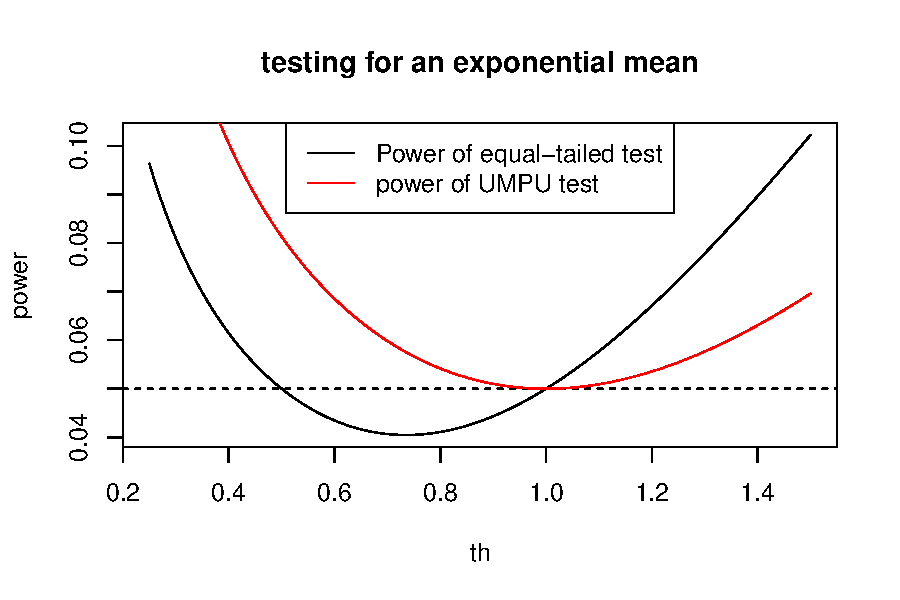
\includegraphics[width=\maxwidth]{figure/unnamed-chunk-7-1} 

}


\end{knitrout}
  
  }
  \end{enumerate}
\item Consider now the case where $Y_1, ..., Y_n$ are iid exponential with mean $\theta$ and we again wish to test $H_0: \theta = \theta_0$ against a two sided $H_1: \theta \neq \theta_0$. The likelihood is:
$$\Pi_{i = 1}^n\rbrac{\frac{1}{\theta}e^{-\frac{Y_i}{\theta}}} = \exp\brac{-\frac{1}{\theta}\sum_{i = 1}^nY_i - n\log\theta}$$
and so clearly $X = \sum_{i = 1}^nY_i$ is a sufficient statistic; indeed this is a 1-parameter exponential family. The UMPU test is thus of the form (3) where $c$ and $d$ are chosen to satisfy the two conditions (4) and (5).

However since $X$ itself has a gamma distribution with shape parameter $n$ and scale parameter $\theta$, the UMPU above is the same as for a single observation from the density (1) above with $\gamma_0 = n$. We show in the tutorial that in the present case the two conditions (4) and (5) are equivalent to
$$ \int_0^cf\brac{x; n, 1}\dx + \int_d^\infty f\brac{x; n, 1}\dx = \alpha = \int_0^c f\brac{x; n + 1, 1}\dx + \int_d^\infty f\brac{x; n + 1, 1}\dx$$

Below we shall write a function to determine the UMPU test, for the case $n = 5$ and $\alpha = 0.05$.
\begin{enumerate}[label=(\alph*)]
  \item By adapting your solution to part (c) of the previous question, write a function (playing the same role as the function \verb+fn()+ above; it will use \verb+pgamma()+ and \verb+qgamma()+) the root of which gives the desired value of $c$ to solve the above equations (\tbf{hint}: in the body of this function you will need to first find \verb+d+ in terms of \verb+c+ and \verb+alpha+ using one of the two constraints). Then use \verb+uniroot()+ to actually find the root. Wrap this all in an appropriate function which takes as input values of \verb+alpha+ and \verb+n+ and outputs a list with elements \verb+c+ and \verb+d+, the lower and upper critical values of the desired UMPU test.
  
  {\setlength{\leftskip}{3ex}
  \tbf{Solution}
  
\begin{knitrout}\footnotesize
\definecolor{shadecolor}{rgb}{0.969, 0.969, 0.969}\color{fgcolor}\begin{kframe}
\begin{alltt}
\hlstd{gamma.root} \hlkwb{=} \hlkwa{function}\hlstd{(}\hlkwc{c}\hlstd{,} \hlkwc{n}\hlstd{,} \hlkwc{alpha}\hlstd{) \{}
    \hlstd{lower} \hlkwb{=} \hlkwd{pgamma}\hlstd{(}\hlkwc{q} \hlstd{= c,} \hlkwc{shape} \hlstd{= n,} \hlkwc{scale} \hlstd{=} \hlnum{1}\hlstd{)}  \hlcom{# P (X < c)}
    \hlcom{# P(X < c) + P(X > d) = alpha P(X > d) = alpha - P(x < c) P(X < d) = 1 - alpha + P(X < c) d =}
    \hlcom{# F^-1(1 - alpha + P(X < c))}
    \hlstd{d} \hlkwb{=} \hlkwd{qgamma}\hlstd{(}\hlkwc{p} \hlstd{=} \hlnum{1} \hlopt{-} \hlstd{alpha} \hlopt{+} \hlstd{lower,} \hlkwc{shape} \hlstd{= n,} \hlkwc{scale} \hlstd{=} \hlnum{1}\hlstd{)}

    \hlcom{# return the equation to solve--> the latter half of the integral equation}
    \hlkwd{return}\hlstd{(}\hlkwd{pgamma}\hlstd{(c,} \hlkwc{shape} \hlstd{= (n} \hlopt{+} \hlnum{1}\hlstd{),} \hlkwc{scale} \hlstd{=} \hlnum{1}\hlstd{)} \hlopt{+} \hlkwd{pgamma}\hlstd{(d,} \hlkwc{shape} \hlstd{= (n} \hlopt{+} \hlnum{1}\hlstd{),} \hlkwc{scale} \hlstd{=} \hlnum{1}\hlstd{,} \hlkwc{lower.tail} \hlstd{=} \hlnum{FALSE}\hlstd{)} \hlopt{-}
        \hlstd{alpha)}
\hlstd{\}}
\end{alltt}
\end{kframe}
\end{knitrout}
Show the roots:
\begin{knitrout}\footnotesize
\definecolor{shadecolor}{rgb}{0.969, 0.969, 0.969}\color{fgcolor}\begin{kframe}
\begin{alltt}
\hlstd{eps} \hlkwb{=} \hlnum{1e-08}
\hlstd{upper} \hlkwb{=} \hlkwd{qgamma}\hlstd{(}\hlnum{0.05}\hlstd{,} \hlkwc{shape} \hlstd{=} \hlnum{5}\hlstd{,} \hlkwc{scale} \hlstd{=} \hlnum{1}\hlstd{)} \hlopt{-} \hlstd{eps}
\hlkwd{uniroot}\hlstd{(}\hlkwc{f} \hlstd{= gamma.root,} \hlkwc{lower} \hlstd{=} \hlnum{0}\hlstd{,} \hlkwc{upper} \hlstd{= upper,} \hlkwc{n} \hlstd{=} \hlnum{5}\hlstd{,} \hlkwc{alpha} \hlstd{=} \hlnum{0.05}\hlstd{)}
\end{alltt}
\begin{verbatim}
## $root
## [1] 1.758069
## 
## $f.root
## [1] 1.352949e-06
## 
## $iter
## [1] 6
## 
## $init.it
## [1] NA
## 
## $estim.prec
## [1] 6.103516e-05
\end{verbatim}
\end{kframe}
\end{knitrout}
And finally wrap all this up in a function:
\begin{knitrout}\footnotesize
\definecolor{shadecolor}{rgb}{0.969, 0.969, 0.969}\color{fgcolor}\begin{kframe}
\begin{alltt}
\hlstd{gamma.umpu} \hlkwb{=} \hlkwa{function}\hlstd{(}\hlkwc{alpha}\hlstd{,} \hlkwc{n}\hlstd{) \{}
    \hlstd{eps} \hlkwb{=} \hlnum{1e-08}
    \hlstd{upper} \hlkwb{=} \hlkwd{qgamma}\hlstd{(alpha,} \hlkwc{shape} \hlstd{= n,} \hlkwc{scale} \hlstd{=} \hlnum{1}\hlstd{)} \hlopt{-} \hlstd{eps}
    \hlstd{c} \hlkwb{=} \hlkwd{uniroot}\hlstd{(}\hlkwc{f} \hlstd{= gamma.root,} \hlkwc{lower} \hlstd{=} \hlnum{0}\hlstd{,} \hlkwc{upper} \hlstd{= upper,} \hlkwc{n} \hlstd{= n,} \hlkwc{alpha} \hlstd{= alpha)}\hlopt{$}\hlstd{root}
    \hlstd{lower} \hlkwb{=} \hlkwd{pgamma}\hlstd{(c,} \hlkwc{shape} \hlstd{= n,} \hlkwc{scale} \hlstd{=} \hlnum{1}\hlstd{)}
    \hlstd{d} \hlkwb{=} \hlkwd{qgamma}\hlstd{(}\hlnum{1} \hlopt{-} \hlstd{(alpha} \hlopt{-} \hlstd{lower),} \hlkwc{shape} \hlstd{= n,} \hlkwc{scale} \hlstd{=} \hlnum{1}\hlstd{)}
    \hlkwd{return}\hlstd{(}\hlkwd{list}\hlstd{(}\hlkwc{c_val} \hlstd{= c,} \hlkwc{d_val} \hlstd{= d))}
\hlstd{\}}
\end{alltt}
\end{kframe}
\end{knitrout}
  
  }
  \item Use your \verb+gamma.umpu()+ function to determine the appropriate $c$ and $d$ for the UMPU test for this problem with $n = 5$ and $\alpha = 0.05$. Plot the power as a function of $\theta$ and graphically verify that the test is unbiased and of level 0.05.
\begin{knitrout}\footnotesize
\definecolor{shadecolor}{rgb}{0.969, 0.969, 0.969}\color{fgcolor}\begin{kframe}
\begin{alltt}
\hlkwd{gamma.umpu}\hlstd{(}\hlnum{0.05}\hlstd{,} \hlnum{5}\hlstd{)}
\end{alltt}
\begin{verbatim}
## $c_val
## [1] 1.758069
## 
## $d_val
## [1] 10.86438
\end{verbatim}
\begin{alltt}
\hlstd{gu} \hlkwb{=} \hlkwd{gamma.umpu}\hlstd{(}\hlnum{0.05}\hlstd{,} \hlnum{5}\hlstd{)}  \hlcom{# obtain c and d}
\hlstd{g.power} \hlkwb{=} \hlkwd{pgamma}\hlstd{(gu}\hlopt{$}\hlstd{c,} \hlkwc{shape} \hlstd{=} \hlnum{5}\hlstd{,} \hlkwc{scale} \hlstd{= th)} \hlopt{+} \hlnum{1} \hlopt{-} \hlkwd{pgamma}\hlstd{(gu}\hlopt{$}\hlstd{d,} \hlkwc{shape} \hlstd{=} \hlnum{5}\hlstd{,} \hlkwc{scale} \hlstd{= th)}
\hlkwd{plot}\hlstd{(th, g.power,} \hlkwc{type} \hlstd{=} \hlstr{"l"}\hlstd{)}
\hlkwd{abline}\hlstd{(}\hlkwc{h} \hlstd{=} \hlnum{0.05}\hlstd{,} \hlkwc{lty} \hlstd{=} \hlnum{2}\hlstd{)}
\end{alltt}
\end{kframe}

{\centering 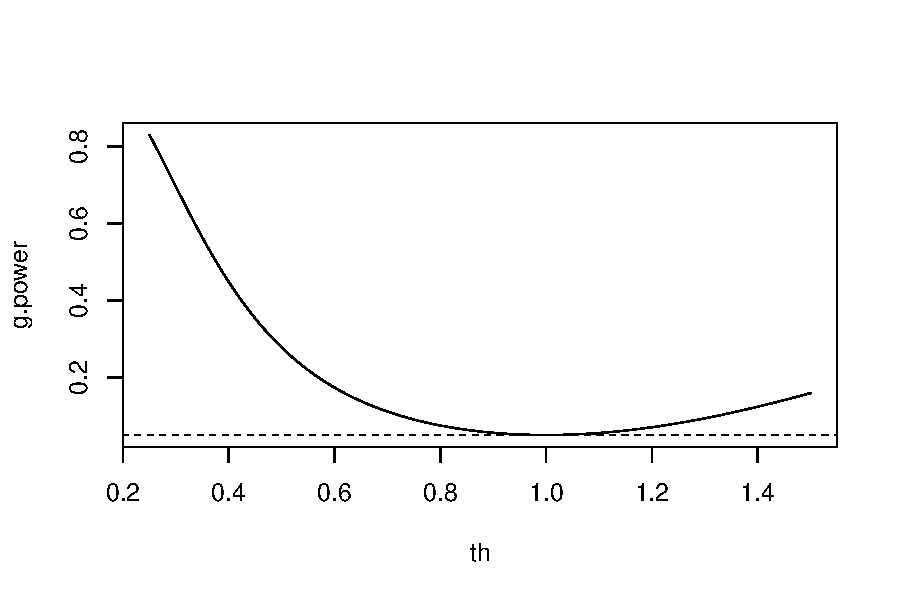
\includegraphics[width=\maxwidth]{figure/unnamed-chunk-11-1} 

}


\end{knitrout}
\end{enumerate}
\end{enumerate}

\newpage

\end{document}
